\chapter{移动机器人的定位与导航}
\label{cha:nav}

定位与导航功能在机器人开发中占有重要地位。一般的,我们认为机器人的定位
导航功能包含环境地图构建、路径规划与运动控制以及自主避障等子任务。Tinker
机器人的定位导航系统基于ROS框架下的Navigation Stack实现,使用激光雷达、
里程计、深度相机等多传感器融合方法,能够完成实时地图构建、重定位、动态
环境下的避障及导航任务。


\section{SLAM算法}

SLAM技术(Simultaneous Localization and Mapping)也称为即时定位与地图构建技术,是一种
依赖各种传感器信息获取机器人位姿以及外部地图的技术。SLAM技术对于在机器人行业十分重要,无论是
目前大规模应用的AGV底盘、送餐机器人还是在实验室中被不断开发的各种操作机器人,任何需要移动的
设备都需要SLAM技术进行辅助。按照依赖的主要传感器可以将SLAM技术粗略的划分为两个方向:激光雷达与
视觉方向。SLAM技术近年来发展十分迅速,在多模态融合方向与传统SLAM与深度信息融合方向的发展十分
活跃。下面本文将大致的介绍经典SLAM领域影响交广的研究方向与方法,并给出本文Tinker机器人使用的
SLAM方案和使用心得。

\subsection{SLAM算法现状与原理分析}

在时间上,基于雷达的SLAM算法出现与成熟都比基于视觉的SLAM技术早一些,其原因是多方面的。笔者认为,
一方面是雷达数据,尤其是单线雷达数据,数据量一般比较小,对计算机性能的需求较低,而实时的处理图片
信息对早年的计算机来说的确是相当困难的一件事;另一方面视觉SLAM的许多辅助工具,例如摄像头标定技术,
合适的特征提取算法与最优化工具以及词袋算法,都是相当晚近才完全成熟的,这在一定程度上拖后了视觉SLAM
技术的发展。

\subsubsection{雷达SLAM技术}

最早被广泛接受的雷达SLAM算法应当是Gmapping\cite{grisettiyz2005improving, grisetti2007improved}。
这是一种基于Rao-Blackwellized滤波的粒子滤波算法,它的输入信息为单线激光雷达和里程计,输出为一张2维
地图以及地图原点同里程计坐标原点的位移,这样我们可以根据里程计信息和gmapping给出的地图原点到里程计原点
的坐标差计算出机器人相对于地图的位置。这样算法就一定程度上利用雷达信息消除了里程计的累计误差,提高了定位
的精度(如图~\ref{fig:gmapping},gmapping建出的MIT Killian Court二维地图)

\begin{figure}
  \centering
  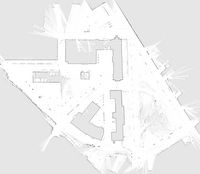
\includegraphics[width=300pt]{gmapping.png}
  \caption{Gmapping建出的MIT Killian Court}
  \label{fig:gmapping}
\end{figure}

得益于其不错的性能和便捷易得的开源实现,gmapping算法在机器人领域得到了广泛的应用,尤其是基于ROS的
机器人生态圈中,gmapping有非常重要的地位。但是gmapping算法本身不支持重定位,即一次建图完成之后
下一次运行时读取之前的地图并得到当前机器人相对之前地图位置的能力。这大大的限制了gmapping在应用时
的方便程度。克服这一缺陷的比较常见的方案是使用AMCL\cite{fox2002kld}(这是一种基于蒙特卡罗模拟
的重定位算法)得到新位置相对于老图的位置,然后使用某些微调技术将新图与老图拼接起来。

雷达SLAM领域十分活跃,有相当多使用不同传感器、不同求解方式的算法不断出现,例如使用单线激光雷达与IMU的
Hector SLAM\cite{KohlbrecherMeyerStrykKlingaufFlexibleSlamSystem2011},适用于多线激光雷达
的LOAM\cite{zhang2014loam}等。

近几年最引人注意的成果是google于2016年发布的Cartographer
\cite{hess2016real},同此前的很多雷达定位算法不同,Cartographer的基本求解思想是基于最优化理论的,
这同前文介绍的基于粒子滤波的gmapping有很大不同。Cartographer还引入了Submap的思想,将大的建图场景
分割成相对较小的子图,在局部匹配和全局匹配时都能发挥较好的作用,如图~\ref{fig:cartographer}为
Cartographer的算法框架。Cartographer同时支持2D与3D激光雷达,且
支持多个雷达组合使用以及雷达与IMU的融合,且原生支持地图重定位和分阶段建图,功能十分全面。早期的Cartographer虽然提供ROS的接口,但是其地图格式没有同ROS中主流的Costmap对接起来,随着社区的发展,将Cartographer同ROS
Navigation Stack对接的轮子越来越完善,Cartographer正在快速替代Gmapping成为开源机器人开发者最常
使用的雷达定位算法。如图\ref{fig:cartographer_map}为Cartographer在德国的Deutsches Museum使用
单线激光雷达建图的结果。

\begin{figure}[h] % use float package if you want it here
  \centering
  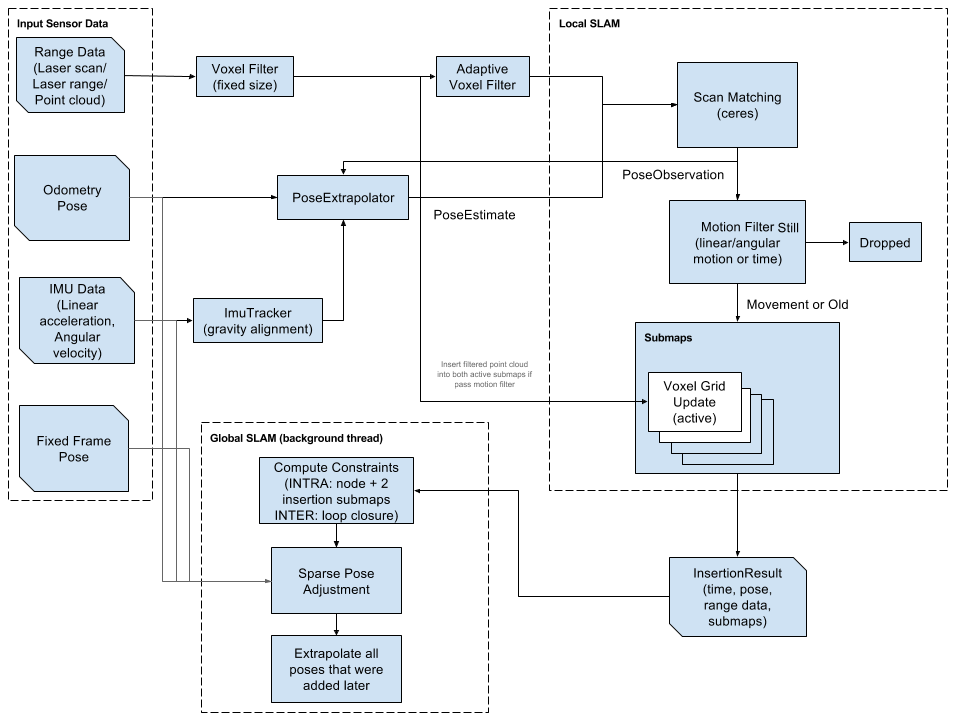
\includegraphics[width=.95\textwidth]{cartographer.png}
  \caption{Cartographer的算法框架}
  \label{fig:cartographer}
\end{figure}

\begin{figure}
  \centering
  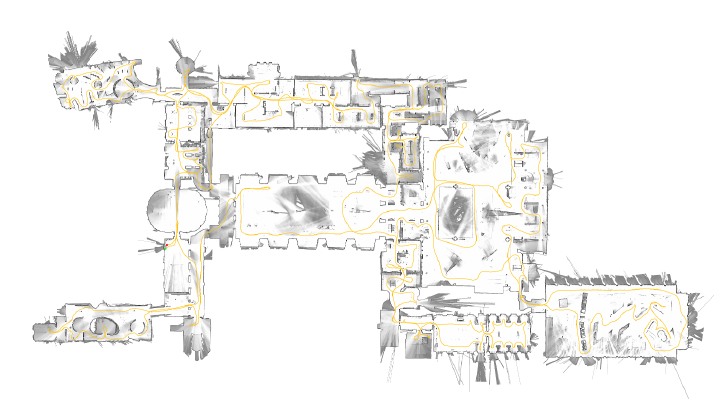
\includegraphics[width=320pt]{cartographer_map.png}
  \caption{Cartographer在Deutsches Museum的建图效果}
  \label{fig:cartographer_map}
\end{figure}



值得一提的,Cartographer中使用的优化框架是Google开发的开源优化器Ceres\cite{ceres-solver},
近几年随着Cartographer等等一些算法的不断出现,Ceres在业内的知名度越来越高,许多基于视觉的SLAM
算法也开始使用Ceres作为优化核心。

\subsubsection{视觉SLAM技术}

视觉SLAM技术的发展更为迅速。从方法上来说可以将视觉SLAM技术笼统的分为直接法、间接法还有半直接法。直接
法是相对于间接法提出的,间接法是指算法在拿到图片后,首先对图片进行特征点提取,然后使用特征点进行后续
的匹配、优化等等过程,因此间接法又被称为特征点法。而直接法是直接使用图片的像素信息进行匹配,一般通过
最小化光度差等等手段进行地图的
重建与位姿提取,而半直接法顾名思意是一种将二者结合的方法。一般直接法对于构建稠密地图有一定优势,但是
专注定位与稀疏建图的算法中还是特征点法占据主流。按照求解思想还可以将视觉SLAM方法划分为使用
优化方法或者滤波方法,目前行业公认优化方法无论在精度、鲁棒性等方面都优于滤波方案。因此本文主要介绍
基于优化的特征点方法中两个具有代表性的算法,以此简要的概括移动操作机器人视觉定位方向的主要形势。

ORB-SLAM算法\cite{mur2015orb}发布时(2015年)在业界引起了很大的震动,这是当时第一款基于特征点
且基本可用的开源单目SLAM算法,在此之前虽然学术界也有一些文章发表,但大多闭源,或者工程实现非常差。
随后一年,原作者又发表并开源了支持双目及RGBD的ORB-SLAM2,ORB-SLAM的影响越来越广泛,可以说这款算法
的发布不但在学术界有极大的影响力,在工业界的震荡也相当大,截止到目前,很多AR企业、基于视觉定位的送餐
机、扫地机等等公司,其核心的定位算法依旧借鉴这款算法开发。ORB-SLAM2算法框架如图~\ref{fig:orb_frame}
所示,在拿到一帧图片后,算法首先对其进行特征提取,特别的这里使用的是ORB特征提取法\cite{rublee2011orb}
,同之前的SIFT、SURF
等等特征提取法不同,ORB算法更适合在CPU上运算,其运算效率比较高,能满足实时性要求。ORB特征点结合了FAST
特征点与Brief描述子,具有方向,且其描述子理论上具有旋转、平移、拉伸不变性,这些特性对于SLAM技术是比较好
的。在完成特征匹配之后,算法会利用描述子将当前帧的特征点与最近的关键帧中的点进行匹配,匹配成功后可以得到
一个粗略
的估计。之后按照一定策略判定当前帧是否是关键帧(例如相邻帧的频率,与上一个关键帧之间的位置差,当前帧的关键
点数等等),如果是的话,要对相关的关键帧再进行一次匹配,以得到可靠的位置约束。在这里ORB-SLAM使用的关键帧
选取策略是共视策略(covisible),即选择在关键帧库中视野与当前帧有交集的那些帧,这种方法相对来说精致一些,
同下文要介绍的VINS有一些不同。上述过程在SLAM领域一般称作Tracking,即追踪过程。为了充分利用环境自带的约束
信息,一般SLAM算法都会在后端运行一个Loop Closing线程,即闭环检测。如图~\ref{fig:loop_closing}所示,
由于累计误差的存在,
在算法运行一段时间视野又回到原点时,其轨迹很可能不会非常理想,但是如果我们能够发现当前的场景和过去的某个
场景有关联,和过去的关键帧建立约束关系,那么此时再对整个轨迹做优化的话,就能很好的消除累计误差,得到不错的
定位效果。ORB SLAM中寻找相似场景主要依赖BoW(Bag of Words,词袋)技术\cite{GalvezTRO12}。基于特征点
与关键帧的ORB-SLAM算法可视化效果如图~\ref{fig:orb_viz}所示,目前大多数基于特征点的SLAM算法都使用
关键帧作为管理点的单位,因此很多算法的可视化效果都和此图差不多。


\begin{figure}[h] % use float package if you want it here
  \centering
  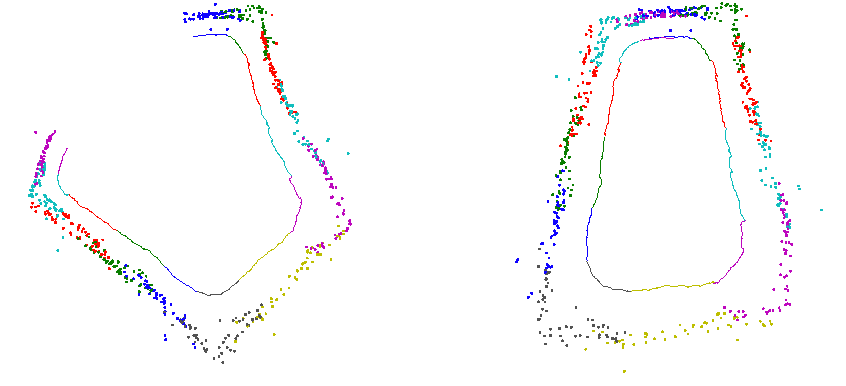
\includegraphics[width=.95\textwidth]{loop_closing.png}
  \caption{应用闭环约束前后的轨迹变化}
  \label{fig:loop_closing}
\end{figure}


\begin{figure}[h] % use float package if you want it here
  \centering
  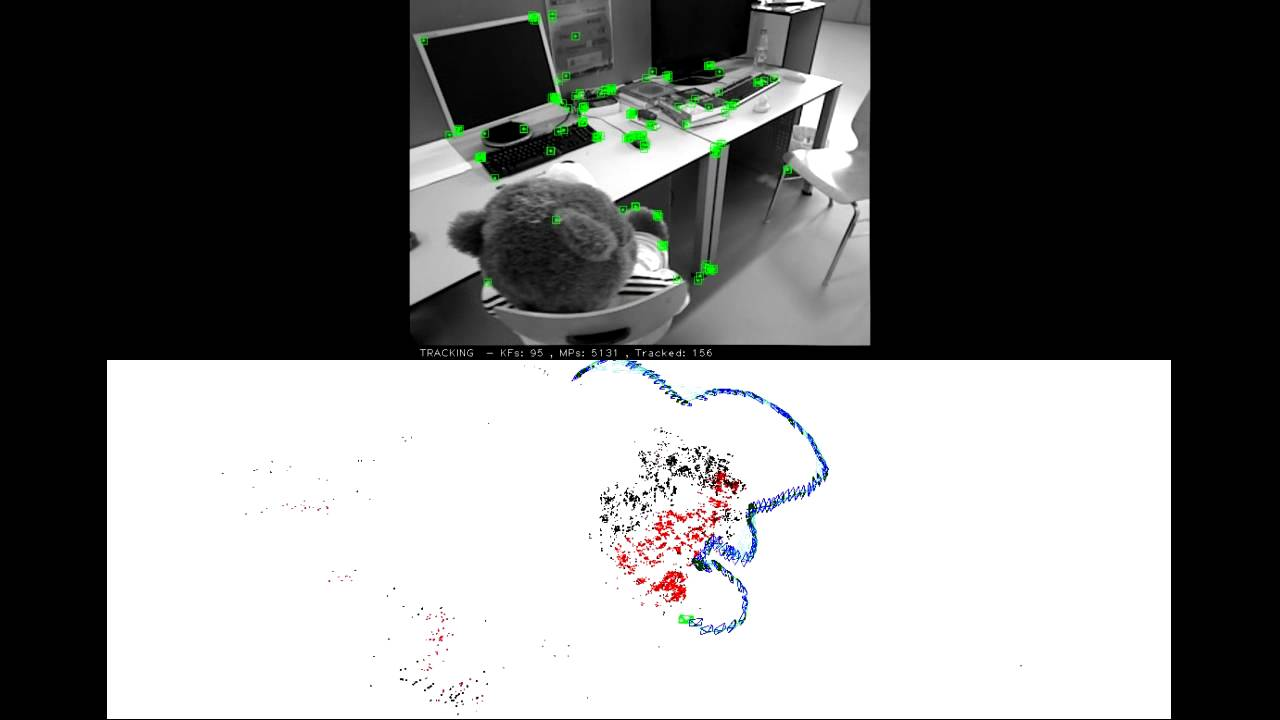
\includegraphics[width=300pt]{orb_viz.jpg}
  \caption{ORB-SLAM运行时的可视化效果}
  \label{fig:orb_viz}
\end{figure}

\begin{figure}[h] % use float package if you want it here
  \centering
  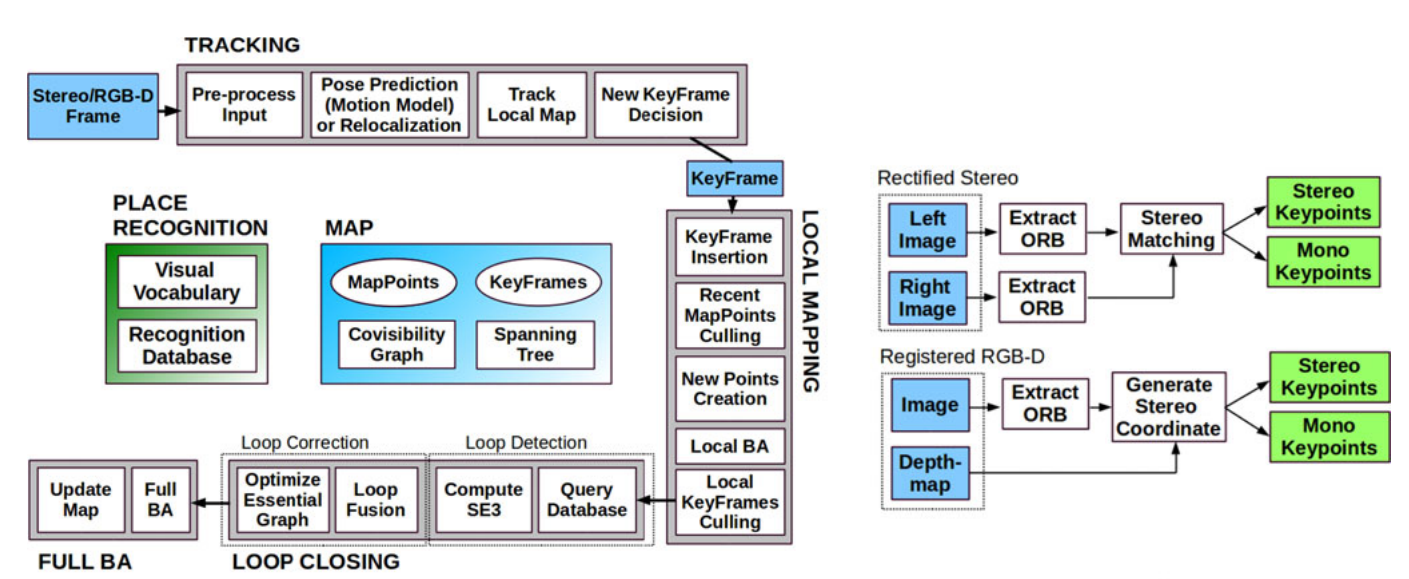
\includegraphics[width=.95\textwidth]{orb_framework.png}
  \caption{ORB-SLAM2的算法框架}
  \label{fig:orb_frame}
\end{figure}




VINS\cite{qin2018vins}算法大致比ORB-SLAM晚2-3年出现,诞生于香港科技大学Shaojie Shen团队,VINS-Mono的发表时间是2018年,VINS-Fusion
稍晚一些,它也是基于优化方案的特征点法SLAM
算法。同ORB-SLAM不同的是,VINS给出了视觉与IMU融合的有效解决方案,有了IMU的辅助VINS在表现上
更加鲁棒,精度也更高,尤其在无人机定位方向表现非常出彩。VINS对IMU数据的一项重要处理手段是IMU预积分
技术(IMU preintegratio),一般认为,这项技术的最早提出是佐治亚理工的C. Foster于2015年发表的
\cite{forster2015imu},而沈的团队于15年发表的\cite{shen2015tightly}就详细的分析了将IMU预积分
应用到无人机的视觉定位算法中的可能性,这篇文章可以视作是VINS的准备工作。如图~\ref{fig:vins_frame}
展示了VINS的算法框架,可以看到VINS的大致工作流程同ORB-SLAM是差不太多的,但是在某些算法方案上有不同。
例如VINS的关键帧选取策略与ORB-SLAM的共视不同,是简单的Sliding Windows方案,即不管当前帧位姿如何
算法都选取临近的若干帧进行位姿优化。这种方案有一定的道理:首先相机是均匀连续移动的这一假设在大多数情况下
都应当是成立的;其次,有IMU数据的修正,算法理论上更加不容易失配,选择相对简单的策略也就是被允许的了。


\begin{figure}[h] % use float package if you want it here
  \centering
  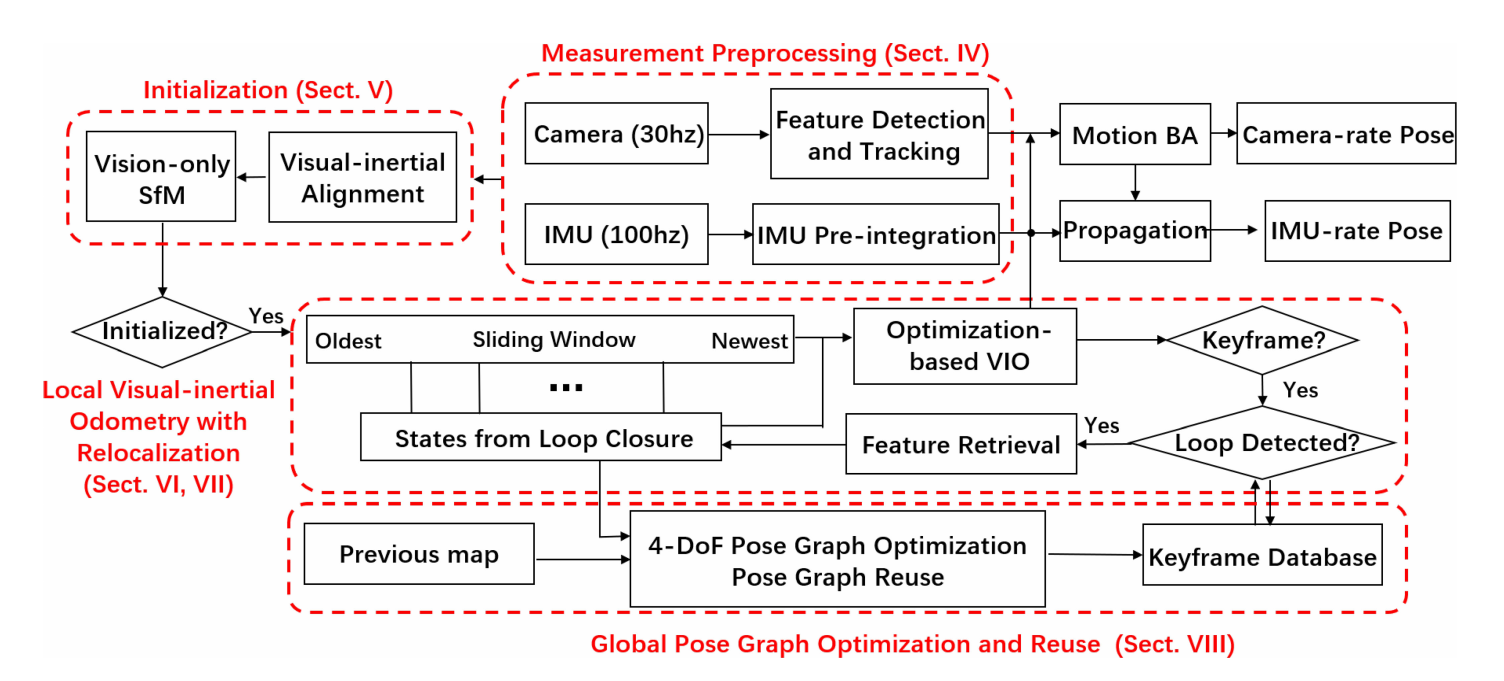
\includegraphics[width=.95\textwidth]{vins_framework.png}
  \caption{VINS-Mono的算法框架}
  \label{fig:vins_frame}
\end{figure}

\subsection{SLAM算法选择与性能分析}


Tinker最初使用的是建图与定位分开实现的方案。建图方面,我们使用
gmapping算法\cite{grisettiyz2005improving},
依赖2个北洋UTM-30LX单线激光雷达拼接定位(如图~\ref{fig:utm30lx})。定位
方面,我们使用基于蒙特卡罗的
amcl算法\cite{fox2002kld},两个算法同时工作时的可视化信息如图~\ref{fig:gmapping_amcl}。
amcl需要在地图已经给出的情况下进行定位,在
真实赛场上,比赛场景多数情况下是确定的,因此这套方案还基本可用,Tinker机器人
会在开赛前对赛场进行扫描,将地图场景保存起来,之后比赛过程中单纯使用amcl
进行定位。后期随着团队成员对这套定位算法越来越熟悉,我们会将场景内可能出现
在单线雷达视野内的一切固定障碍的尺寸量下来,使用绘图软件对地图进行重建,然后
使用amcl进行定位,可以拿到更好的定位效果。

\begin{figure}
  \centering
  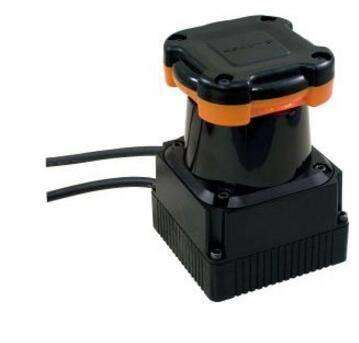
\includegraphics[width=150pt]{utm30lx.jpeg}
  \caption{北洋UTM-30LX单线激光雷达}
  \label{fig:utm30lx}
\end{figure}


\begin{figure}
  \centering
  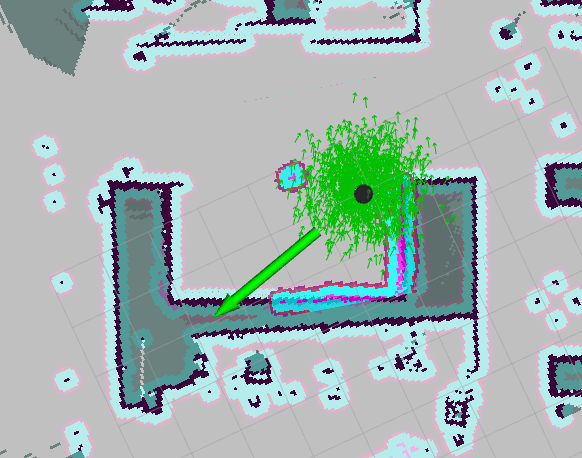
\includegraphics[width=300pt]{gmapping_amcl.png}
  \caption{Gmapping + Amcl可视化效果}
  \label{fig:gmapping_amcl}
\end{figure}

虽然上述方案在长时间内被证明是稳定可用的,但随着SLAM社区的不断发展,基于
粒子滤波的定位建图算法已经过时了,尤其是Google开源其自主开发的Cartographer
雷达建图定位算法\cite{hess2016real}之后,本工作后期也将定位方案迁移为Cartographer+
ROS Navigation的模式,在更换建图定位算法之后,配合我们对Tinker硬件的二次
改版,我们也将原有的2个单线雷达减少为一个,变动之后定位数据减少,运算效率也
得到了提升。Cartographer的算法框架如图~\ref{fig:cartographer}所示。


除了基于单线激光雷达的各种定位建图算法外,笔者还尝试了一些基于特征点的视觉SLAM
方案,例如基于ORB特征点法的ORB-SLAM2(使用Kinect v2的RGB-D数据)\cite{mur2015orb},
ORB-SLAM2在室内环境中的可视化效果如图TODO所示。我们还测试了基于双目和IMU数据
融合的VINS-Fusion\cite{qin2018vins}算法,并且分析了两算法表现上的差异。

ORB-SLAM2的算法框架如图~\ref{fig:orb_frame}所示,其获取到原始数据后,首先对左右
目的图像提取特征,完成三角化,之后使用特征点的描述子在关键帧库中选取合适的帧
进行匹配,ORB-SLAM的关键帧选取策略较复杂,是一种基于共视关系的选取方案,即我们
在仓库中选取可能和当前帧看到同一场景的帧来进行匹配,在完成局部位姿优化后,经过
关键帧筛选策略选取关键帧,之后后端不断尝试通过词袋法发现相同场景,完成大的闭环
优化。VINS的算法框架如图~\ref{fig:vins_frame}所示,vins也是基于关键点法进行位姿
匹配的算法,同ORB-SLAM的主要区别有两个:一是VINS有IMU融合,其处理IMU数据的方式
为IMU预积分(IMU preintegration)\cite{forster2015manifold},且它将处理结果作为
优化项中的一个因子参与了位姿优化;二是VINS的
关键帧选择策略是简单的Sliding Window算法,即选取与当前帧在时间上相邻的几个关键帧
进行特征匹配与优化,这个策略和ORB-SLAM的共视图策略想比较略显粗糙,但是在大场景
下还是有不错的匹配效果。




\section{导航方案的选择}

Tinker的开发过程中一直使用ROS作为主要开发框架,而ROS的Navigation Stack中对于
导航避障提供了一套较为成熟的解决方案。Tinker前后使用了2套定位与规划算法,下面两个
章节中将对这两套方案进行详细描述。

\subsection{路径规划}

ROS的Navigation stack中提供了一整套导航避障的解决方案。其核心是同时维护地图信息
与路径规划器。地图信息使用一种分层管理的方式\cite{lu2014layered},并且分别维护
全局地图 Global Map与局部地图 Local Map。规划器也有两个,分别是Global Planner
和Local Planner。其中 Global Planner负责根据全局地图生成路径,而 Local Planner
则负责根据局部地图生成速度指令,传输给底盘执行。Tinker使用的 Global Planner是
一种基于 Dijkstra算法\cite{deng2012fuzzy}的路径生成方法,Local Planner是
一种基于dynamic window approach的速度生成方案\cite{fox1997dynamic}如图,其算法思想
为:在当前位置向各个方向以不同速度发射模拟路径,并且按照这些路径是否经过障碍物、
离目标路径的远近等等条件本别进行打分,选取分数最高的路径对应的速度极为dwa的输出
结果~\ref{fig:dwa}。上述
方案均为机器人导航领域较为经典且通用的方案,本工作对上述算法进行了一些微调,以
使算法在Tinker平台上有更好的表现,如图~\ref{nav_costmap}所示为Tinker进行导航任
务时可视化的调试信息。


\begin{figure}[h] % use float package if you want it here
  \centering
  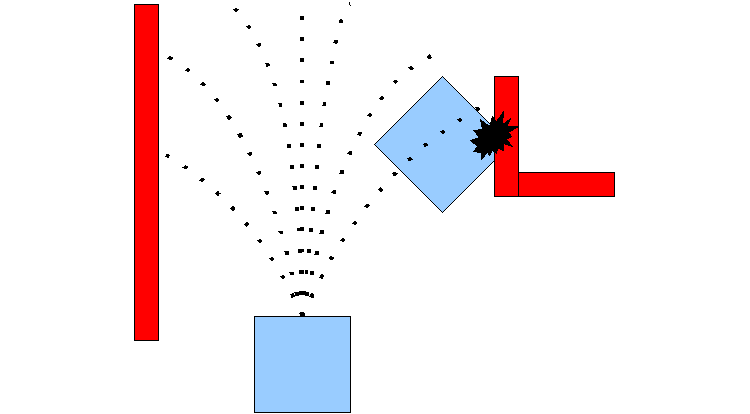
\includegraphics[width=1.\textwidth]{dwa.png}
  \caption{dwa算法示意图}
  \label{fig:dwa}
\end{figure}


\begin{figure}[h] % use float package if you want it here
  \centering
  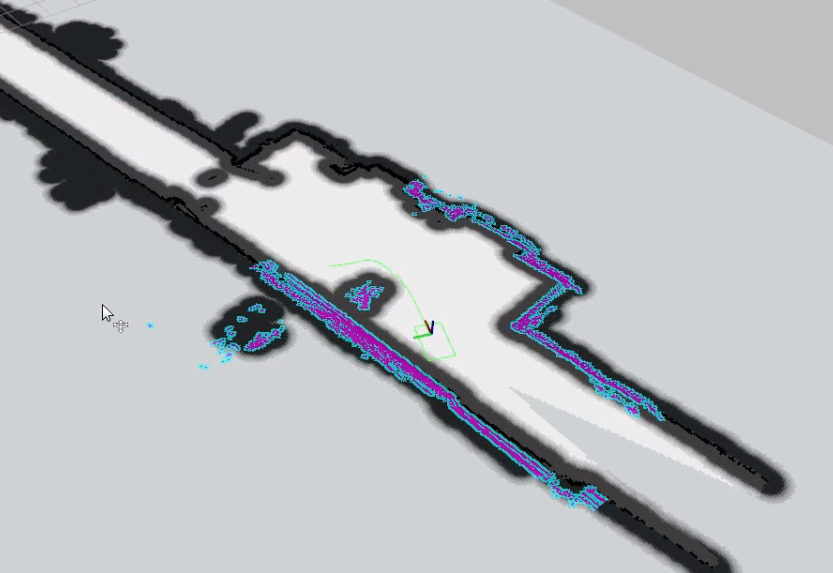
\includegraphics[width=1.\textwidth]{nav_costmap.png}
  \caption{进行导航任务时的地图与路径}
  \label{fig:nav_costmap}
\end{figure}

\subsection{机器人控制}

由于Tinker机器人使用全向麦克纳姆轮底盘,且每个电机控制一个麦轮,其运动学解算同
传统2轮底盘或者4轮阿克曼转向底盘相比更复杂一些。


\begin{figure}[h] % use float package if you want it here
  \centering
  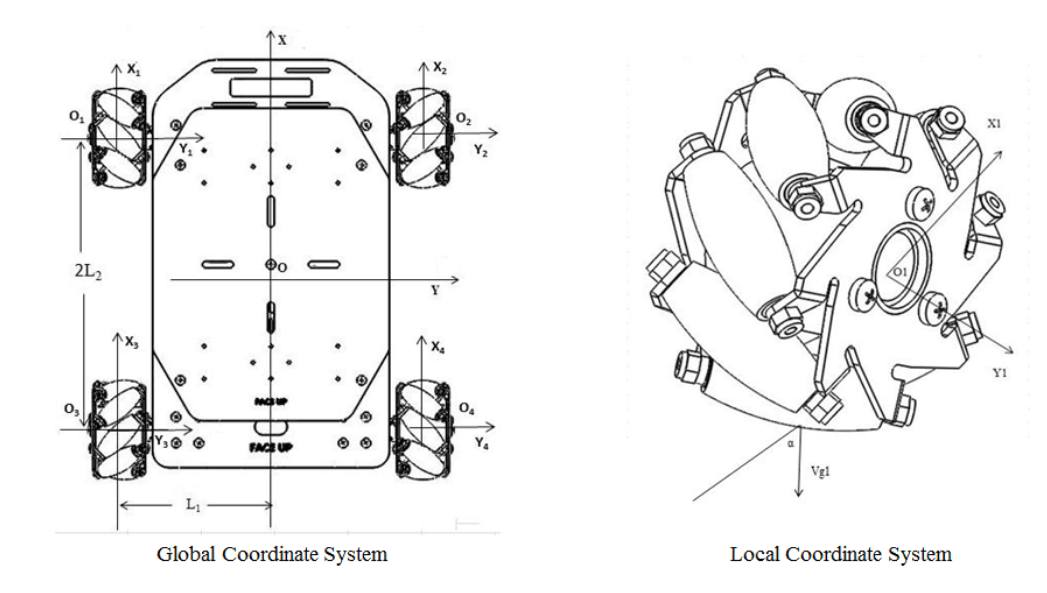
\includegraphics[width=.95\textwidth]{mecanum.png}
  \caption{麦轮底盘(左)与麦轮放大图(右),图片来源\cite{mecanum}}
  \label{fig:mecanum}
\end{figure}

如图~\ref{fig:mecanum}所示,假设底盘麦轮X型安装,其4轮到底盘中心的横向纵向距离分别
为$L_1$、$L_2$,四个车轮的转速为$\omega_1$、$\omega_2$、$\omega_3$、$\omega_4$
(即为电机转速),四个车轮上滚子的速度分别为$v_{g1}$、$v_{g2}$、$v_{g3}$、$v_{g4}$,
四个轮子的主轴的瞬时速度为$v_{O1x}, v_{O1y}$,$v_{O2x}, v_{O2y}$,$v_{O3x}, v_{O3y}$,
$v_{O4x}, v_{O4y}$,整个底盘的速度可表示为$v_x, v_y, \omega_O$,麦轮滚子轴与麦轮主轴
的夹角为$\alpha$(一般为\ang{45}),麦轮滚子轴到主轴的距离为$R$

根据速度分解,对1轮可列出~\ref{equ:glo_vec};对单个麦轮进行速度分析,可得~\ref{equ:loc_vec}

\begin{equation}
  \label{equ:glo_vec}
  \begin{aligned}
    v_{O1x} = v_x - \omega_O * L_1\\
    v_{O1y} = v_y - \omega_O * L_2
  \end{aligned}
\end{equation}

\begin{equation}
  \label{equ:loc_vec}
  \begin{aligned}
    v_{O1x} &= - v_{g1} * \cos\alpha + \omega_1 * R\\
    v_{O1y} &= v_{g1} * \sin\alpha
  \end{aligned}
\end{equation}

将~\ref{equ:glo_vec}~\ref{equ:loc_vec}两式联立消去轮速,可得~\ref{equ:mid_equ},
将两式合并消去$v_{g1}$,最终得到~\ref{equ:fin_equ}。

\begin{equation}
  \label{equ:mid_equ}
  \begin{aligned}
    v_x - \omega_O * L_1 &= - v_{g1} * \cos\alpha + \omega_1 * R \\
    v_y - \omega_O * L_2 &= v_{g1} * \sin\alpha
  \end{aligned}
\end{equation}


\begin{equation}
  \label{equ:fin_equ}
  \omega_1 = \frac{1}{R}
    \begin{bmatrix}
      1 & \frac{1}{\tan\alpha} & -(L_1 + \frac{L_2}{\tan\alpha})
    \end{bmatrix}
    \begin{bmatrix}
      v_x \\
      v_y \\
      \omega_O
    \end{bmatrix}
\end{equation}

因为此处$\alpha$取值为\ang{45},将其带入后可以得到四个轮子的电机输出转速与目标速度的转换
公式为\ref{equ:fin_all}

\begin{equation}
  \label{equ:fin_all}
  \begin{bmatrix}
    \omega_1 \\
    \omega_2 \\
    \omega_3 \\
    \omega_4
  \end{bmatrix}
    = \frac{1}{R}
  \begin{bmatrix}
    1 &  1 & -(L_1 + L_2) \\
    1 & -1 &  (L_1 + L_2) \\
    1 & -1 & -(L_1 + L_2) \\
    1 &  1 &  (L_1 + L_2) \\
  \end{bmatrix}
  \begin{bmatrix}
    v_x \\
    v_y \\
    \omega_O
  \end{bmatrix}
\end{equation}

值得一提的是通过不断探索,作者发现:在底盘接受速度命令端加一个smoother,对临近的
几帧速度命令进行一定程度的加权平滑(即一个一阶低通滤波器)~\ref{equ:filter}能够使
机器人的运动性能得到质的提升,本文使用的一阶低通滤波算法如下:

\begin{equation}
  \label{equ:filter}
  v_{final} = 0.9 * v_{origin} + 0.1 * v_{cur}
\end{equation}

这一发现也提示我们,对于机器人这一复杂系统来说,提升整体性能的手段是多元的,在制
定方案时应勇于尝试
多做实验,积极尝试各种想法,这样有助于我们使用较低的成本达到更好的性能。

\section{本章小结}

本章较为概括的描述了机器人定位导航领域的大致现状,并且选取了领域内具有划时代意义且目前依然
使用广泛的几个算法进行重点介绍;同时,本章完整的给出了Tinker机器人移动定位导航方向使用的
方案以及开发过程中的经验教训。

下一章,本文将介绍移动操作机器人的重点技术——视觉检测与机械臂规划。




